\documentclass{article}

\usepackage[hungarian]{babel}
\usepackage{mathptmx} % Times New Roman font
\usepackage{titlesec} % For customizing section titles
\usepackage{ragged2e} % For justified text alignment
\usepackage{setspace} % For line spacing
\usepackage[margin=2.5cm]{geometry} % Margin settings
\usepackage[hidelinks]{hyperref} % Enable hyperlinks in TOC
\usepackage{graphicx}

% Set section to 14pt font size
\titleformat{\section}
  {\normalfont\fontsize{14}{16}\bfseries}{\thesection}{1em}{}

% Set subsection to 12pt font size
\titleformat{\subsection}
  {\normalfont\fontsize{12}{14}\bfseries}{\thesubsection}{1em}{}

\begin{document}
    \onehalfspacing % Set line spacing to 1.5
    \justifying % Justify text alignment

    \begin{titlepage}
        \centering
        \vspace*{0.25\textheight}
        {\fontsize{64}{32}\bfseries Jegyzőkönyv \par}
        \vspace{1.5em}
        {\fontsize{25}{64}\normalfont Webes adatkezelő környezetek \par}
        \vspace{1em}
        {\fontsize{25}{32}\normalfont Féléves feladat \par}
        \vspace{1em}
        {\fontsize{25}{32}\normalfont A feladat címe \par}
        \vspace*{0.20\textheight}

        \begin{flushright}
            \begin{tabular}{@{}l@{}}
                {\fontsize{14}{14}\normalfont Készítette: Orosz Péter} \\
                {\fontsize{14}{14}\normalfont Neptun kód: WO02D7} \\
                {\fontsize{14}{14}\normalfont Dátum: ....-..-..} \\
            \end{tabular}
        \end{flushright}
    \end{titlepage}

    \tableofcontents
    \newpage

    \section*{Bevezetés}
    \addcontentsline{toc}{section}{Bevezetés}

    \section*{A feladat leírása}
    \addcontentsline{toc}{section}{A feladat leírása}

    \section{Első feladat címe}
  \subsection{Az adatbázis ER modell tervezése}
    Az adatbázis szerkezetét az ER diagram szemlélteti (lásd az alábbi ábrát), amelyben az entitások, attribútumok és kapcsolatok kerültek megtervezésre. Az ER modell célja, hogy áttekinthetően ábrázolja az adatbázis logikai felépítését, a főbb adatcsoportokat és azok összefüggéseit.

    \begin{figure}[h!]
      \centering
      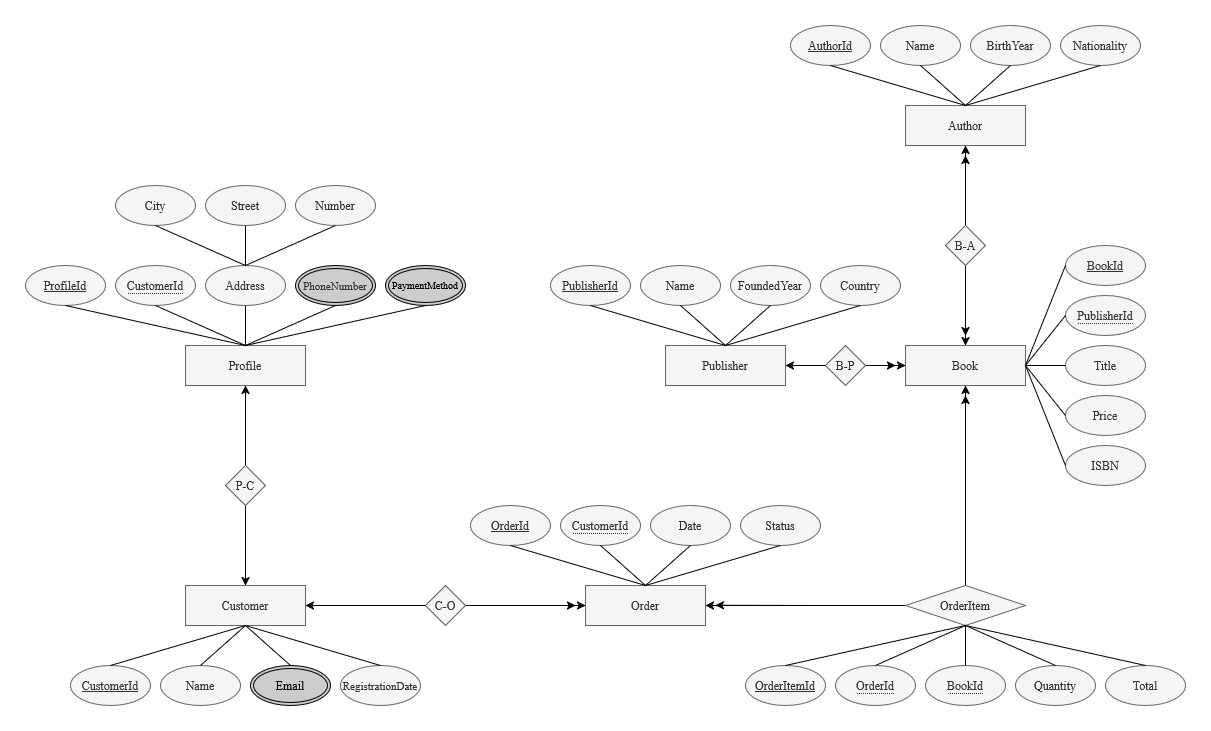
\includegraphics[width=0.85\textwidth]{WO02D7_ER.jpg}
      \caption{Az adatbázis ER diagramja}
    \end{figure}

    \subsubsection*{Entitások és attribútumaik}
  \begin{center}
  \begin{tabular}{|l|l|l|l|}
  \hline
  	\textbf{Entitás} & \textbf{Főkulcs} & \textbf{Idegen kulcs(ok)} & \textbf{Attribútum(ok) (típus)} \\
  \hline
  Profile & ProfileId & CustomerId & Address: City (egyszeres) \\
   &  &  & Address: Street (egyszeres) \\
   &  &  & Address: Number (egyszeres) \\
   &  &  & PhoneNumber (többszörös) \\
   &  &  & PaymentMethod (többszörös) \\
  \hline
  Customer & CustomerId & -- & Name (egyszeres) \\
   &  &  & Email (többszörös) \\
   &  &  & RegistrationDate (egyszeres) \\
  \hline
  Order & OrderId & CustomerId & Date (egyszeres) \\
   &  &  & Status (egyszeres) \\
  \hline
  OrderItem & OrderItemId & OrderId, BookId & Quantity (egyszeres) \\
   &  &  & Total (egyszeres) \\
  \hline
  Book & BookId & PublisherId & Title (egyszeres) \\
   &  &  & Price (egyszeres) \\
   &  &  & ISBN (egyszeres) \\
  \hline
  Author & AuthorId & -- & Name (egyszeres) \\
   &  &  & BirthYear (egyszeres) \\
   &  &  & Nationality (egyszeres) \\
  \hline
  B-A & -- & BookId, AuthorId & -- \\
  \hline
  Publisher & PublisherId & -- & Name (egyszeres) \\
   &  &  & FoundedYear (egyszeres) \\
   &  &  & Country (egyszeres) \\
  \hline
  \end{tabular}
  \end{center}

  \subsection{Az adatbázis konvertálása XDM modellre}
    Az ER diagram alapján elkészült az XDM modell (lásd az alábbi ábrát), amely az adatszerkezetet XML-re optimalizált formában mutatja be. Az XDM modell segíti az XML dokumentum struktúrájának megtervezését, figyelembe véve az adatok hierarchiáját és összefüggéseit.

    \begin{figure}[h!]
      \centering
      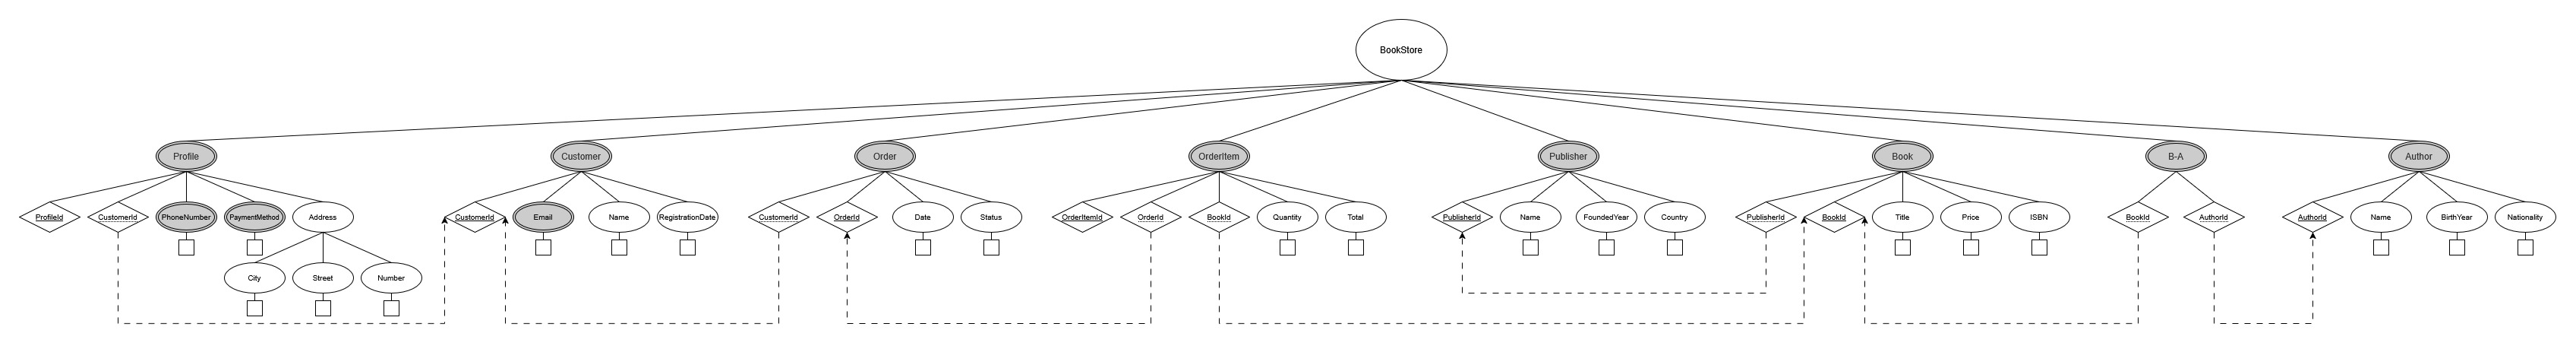
\includegraphics[width=0.85\textwidth]{WO02D7_XDM.jpg}
      \caption{Az adatbázis XDM modellje}
    \end{figure}

  \newpage
  \subsection{Az XDM modell alapján XML dokumentum készítése}
    Az XDM modellből kiindulva elkészült az XML dokumentum (lásd: \texttt{WO02D7\_XML.xml}), amely az adatok tényleges tárolását biztosítja. Az XML fájlban az adatok a modellnek megfelelően hierarchikusan, jól strukturáltan jelennek meg.

    \begin{verbatim}
<?xml version="1.0" encoding="UTF-8"?>
<BookStore>
  <Customer CustomerId="C001">
    <Name>John Doe</Name>
    <Email>john.doe@example.com</Email>
    <RegistrationDate>2022-01-15</RegistrationDate>
  </Customer>
  ...
</BookStore>
    \end{verbatim}

    Az XML dokumentum szerkezete lehetővé teszi több vevő, profil, rendelés, szerző, kiadó és könyv kezelését, valamint az adatok közötti kapcsolatok megjelenítését.

  \subsection{Az XML dokumentum alapján XMLSchema készítése}
        Az XML dokumentum szerkezetének validálásához elkészült az XMLSchema (lásd: \texttt{WO02D7\_XMLSchema.xsd}), amely meghatározza az elemek típusait, kötelező és opcionális mezőket, valamint az adatok közötti kapcsolatokat. Az XMLSchema biztosítja, hogy az XML dokumentum megfeleljen a kívánt szerkezeti és tartalmi követelményeknek.

        \begin{verbatim}
<xs:element name="Customer" maxOccurs="unbounded">
  <xs:complexType>
    <xs:sequence>
      <xs:element name="Name" type="xs:string"/>
      <xs:element name="Email" type="EmailType" maxOccurs="unbounded"/>
      <xs:element name="RegistrationDate" type="xs:date"/>
    </xs:sequence>
    <xs:attribute name="CustomerId" type="xs:string" use="required"/>
  </xs:complexType>
</xs:element>

<xs:simpleType name="EmailType">
  <xs:restriction base="xs:string">
    <xs:pattern value="[a-zA-Z0-9._%+-]+@[a-zA-Z0-9.-]+\.[a-zA-Z]{2,}"/>
  </xs:restriction>
</xs:simpleType>
        \end{verbatim}

        Az XMLSchema részleteiben megtalálhatók az egyedi típusdefiníciók, mint például az email címek, telefonszámok, fizetési módok és státuszok mintái, amelyek biztosítják az adatok helyességét és konzisztenciáját.
\end{document}